
\documentclass[11pt]{article}

\usepackage[margin=0.9in]{geometry}
\usepackage{amsmath,amssymb}
\usepackage{array}
\usepackage{booktabs}
\usepackage{enumitem}
\usepackage{listings}
\usepackage{xcolor}
\usepackage{tikz}
\usepackage{hyperref}

\usetikzlibrary{arrows.meta,positioning,calc}

\definecolor{backcolour}{rgb}{0.95,0.95,0.92}
\definecolor{codeblue}{rgb}{0.05,0.15,0.55}
\definecolor{codegreen}{rgb}{0.0,0.45,0.0}

\lstset{
    backgroundcolor=\color{backcolour},
    basicstyle=\ttfamily\small,
    keywordstyle=\color{codeblue}\bfseries,
    commentstyle=\color{codegreen},
    stringstyle=\color{purple},
    breaklines=true,
    frame=single,
    showstringspaces=false,
    tabsize=4
}

\title{CPSC 250 \\ Big Program One: Constructing a 32-Bit Floating Point Representation}
\author{Edward Brash}
\date{}

\begin{document}

\maketitle

\section{Purpose of the Program}

In this set of notes, we will build a larger Python program whose purpose is to illustrate how a real number can be represented in binary floating point form.

The goal is not to replace Python's built-in floating point system. Python already does this for us. Instead, the goal is pedagogical:

\begin{quote}
We want to understand, step by step, how a decimal floating point number can be decomposed into a binary representation involving a sign bit, exponent bits, and mantissa bits.
\end{quote}

This program brings together many of the ideas reviewed earlier in the course.

\section{Skills Needed}

To build this program, we will need several pieces of Python knowledge.

\begin{enumerate}
    \item Knowledge of primitive data types: integers, floats, and strings.
    \item Knowledge of functions: functions we write ourselves, built-in functions, and class methods.
    \item Knowledge of how floating point numbers are stored.
    \item Loops: both \texttt{for} loops and \texttt{while} loops.
    \item Branching: \texttt{if}, \texttt{else}, and logical conditions.
    \item Getting input from the user.
    \item Producing formatted output using \texttt{print()}.
\end{enumerate}

\section{Overall Program Design}

The program will ask the user for a decimal floating point number, then construct an approximate binary floating point representation.

The high-level design is:

\begin{enumerate}
    \item Get a floating point number from the user.
    \item Ask how many binary places should be used after the binary point.
    \item Write a function that converts the integer part of the number to binary.
    \item Write a function that converts the fractional part of the number to binary.
    \item Determine the mantissa and exponent.
    \item Construct a 32-bit floating point representation.
\end{enumerate}

\section{Step 1: Get a Floating Point Number}

We begin by asking the user for a decimal floating point value.

\begin{lstlisting}[language=Python]
n = input("Enter your floating point value: ")
\end{lstlisting}

Important:

\begin{quote}
The value returned by \texttt{input()} is always a string.
\end{quote}

Therefore, if the user enters \texttt{3.125}, then initially Python stores the text string \texttt{"3.125"}, not the numeric value \texttt{3.125}. To treat this value numerically, we convert it:

\begin{lstlisting}[language=Python]
n = float(input("Enter your floating point value: "))
\end{lstlisting}

\section{Step 2: Ask for the Number of Binary Decimal Places}

Next, we ask how many places should be included after the binary point.

For example, the decimal number

\[
0.1_{10}
\]

has a binary expansion that does not terminate cleanly:

\[
0.1_{10} = 0.0001100110011\ldots_2
\]

Therefore, in a practical program, we must decide how many binary digits after the point we want to keep.

\begin{lstlisting}[language=Python]
p = int(input("Enter the number of binary places in the result: "))
\end{lstlisting}

The variable \texttt{p} is an integer. For example, if \texttt{p = 6}, then we will compute six binary digits after the binary point.

\section{Step 3: Write a Conversion Function}

We want to write a function that takes the number \texttt{n} and the number of binary places \texttt{p}, then returns the binary representation as a string.

\begin{lstlisting}[language=Python]
def get_binary_rep(n, p):
    ...
    return result
\end{lstlisting}

The output will be a string because binary representations such as \texttt{11.001000} are easiest to construct as text.

\section{Working Example}

We will use:

\[
3.125_{10}
\]

and compute the binary representation to six places after the binary point.

\[
3.125_{10} = 11.001000_2
\]

The rest of these notes explain how to produce this result algorithmically.

\section{Breaking the Problem into Pieces}

To convert a decimal number to binary, we separate it into two parts:

\[
3.125 = 3 + 0.125
\]

Then we handle each part separately:

\begin{enumerate}
    \item Convert the integer part to binary.
    \item Convert the fractional part to binary.
    \item Join the two pieces with a binary point.
\end{enumerate}

\section{Converting the Integer Part to Binary}

For the integer part:

\[
3_{10} = 11_2
\]

More generally, we convert an integer to binary using repeated integer division by 2.

\subsection{Example: Converting 13 to Binary}

Consider:

\[
13_{10}
\]

We repeatedly divide by 2 and track the remainder.

\begin{center}
\begin{tabular}{ccc}
\toprule
Number & Integer Division by 2 & Remainder \\
\midrule
13 & 13 // 2 = 6 & 13 \% 2 = 1 \\
6  & 6 // 2 = 3  & 6 \% 2 = 0 \\
3  & 3 // 2 = 1  & 3 \% 2 = 1 \\
1  & 1 // 2 = 0  & 1 \% 2 = 1 \\
\bottomrule
\end{tabular}
\end{center}

The remainders are produced from right to left:

\[
13_{10} = 1101_2
\]

\subsection{Algorithm}

The algorithm is:

\begin{enumerate}
    \item Start with an integer \texttt{num}.
    \item Set the result string to the empty string.
    \item While \texttt{num > 0}:
    \begin{enumerate}
        \item Compute \texttt{digit = num \% 2}.
        \item Add this digit to the front of the result string.
        \item Replace \texttt{num} with \texttt{num // 2}.
    \end{enumerate}
\end{enumerate}

\subsection{Python Function}

\begin{lstlisting}[language=Python]
def convert_integer_to_binary(num):
    # Convert a nonnegative integer to a binary string.

    if num == 0:
        return "0"

    result = ""

    while num > 0:
        digit = num % 2
        result = str(digit) + result
        num = num // 2

    return result
\end{lstlisting}

The line

\begin{lstlisting}[language=Python]
result = str(digit) + result
\end{lstlisting}

adds the new digit to the front of the string because the remainders appear in reverse order.

\section{Converting the Fractional Part to Binary}

Now consider the fractional part:

\[
0.125_{10}
\]

Since

\[
0.125 = \frac{1}{8},
\]

we know:

\[
0.125_{10} = 0.001_2
\]

To six places:

\[
0.125_{10} = 0.001000_2
\]

\section{Understanding Binary Fractions}

Binary fractional places represent powers of two:

\[
0.b_1b_2b_3b_4\ldots_2
\]

means:

\[
b_1\left(\frac{1}{2}\right)
+
b_2\left(\frac{1}{4}\right)
+
b_3\left(\frac{1}{8}\right)
+
b_4\left(\frac{1}{16}\right)
+\cdots
\]

So:

\[
0.001_2 = 0\left(\frac{1}{2}\right)
+0\left(\frac{1}{4}\right)
+1\left(\frac{1}{8}\right)
=
0.125_{10}
\]

\section{Hand Algorithm for the Fractional Part}

For a fractional number, compare it to:

\[
\frac{1}{2}, \frac{1}{4}, \frac{1}{8}, \frac{1}{16}, \ldots
\]

At each step:

\begin{itemize}
    \item If the current number is greater than or equal to the comparison value, write \texttt{1} and subtract the comparison value.
    \item Otherwise, write \texttt{0}.
\end{itemize}

\subsection{Example: 0.125}

To six places:

\begin{center}
\begin{tabular}{cccc}
\toprule
Place & Comparison & Current Number & Output Bit \\
\midrule
1 & $1/2 = 0.5$      & 0.125 & 0 \\
2 & $1/4 = 0.25$     & 0.125 & 0 \\
3 & $1/8 = 0.125$    & 0.125 & 1 \\
4 & $1/16 = 0.0625$  & 0     & 0 \\
5 & $1/32 = 0.03125$ & 0     & 0 \\
6 & $1/64 = 0.015625$& 0     & 0 \\
\bottomrule
\end{tabular}
\end{center}

Thus:

\[
0.125_{10} = 0.001000_2
\]

\subsection{Example: 0.95}

For a less trivial example:

\[
0.95_{10}
\]

\begin{itemize}
    \item $0.95 > 0.5$, so write 1 and subtract:
    \[
    0.95 - 0.5 = 0.45
    \]
    \item $0.45 > 0.25$, so write 1 and subtract:
    \[
    0.45 - 0.25 = 0.20
    \]
    \item $0.20 > 0.125$, so write 1 and subtract:
    \[
    0.20 - 0.125 = 0.075
    \]
    \item $0.075 > 0.0625$, so write 1 and subtract:
    \[
    0.075 - 0.0625 = 0.0125
    \]
\end{itemize}

So the binary fraction begins:

\[
0.95_{10} \approx 0.1111\ldots_2
\]

The expansion continues, and because many decimal fractions do not terminate in binary, this process often produces an approximation.

\section{Python Function for the Fractional Part}

\begin{lstlisting}[language=Python]
def convert_fraction_to_binary(num, places):
    # Convert the fractional part of a number to binary.

    result = ""
    count = 0

    while num > 0 and count < places:
        comparison = 2 ** (-(count + 1))

        if num >= comparison:
            result = result + "1"
            num = num - comparison
        else:
            result = result + "0"

        count = count + 1

    while len(result) < places:
        result = result + "0"

    return result
\end{lstlisting}

\section{Putting the Pieces Together}

Now we combine the integer and fractional pieces.

\begin{lstlisting}[language=Python]
def get_binary_rep(n, p):
    # Return a binary string representation of n using p fractional bits.

    front = int(n)
    back = n - front

    front_bin = convert_integer_to_binary(front)
    back_bin = convert_fraction_to_binary(back, p)

    result = front_bin + "." + back_bin

    return result
\end{lstlisting}

For:

\begin{lstlisting}[language=Python]
get_binary_rep(3.125, 6)
\end{lstlisting}

the result is:

\begin{lstlisting}
11.001000
\end{lstlisting}

\section{From Binary Representation to Floating Point Form}

Once we have a binary representation such as:

\[
11.001000_2
\]

we want to express it in normalized binary scientific notation:

\[
1.xxxxx \times 2^E
\]

For example:

\[
11.001000_2 = 1.1001000_2 \times 2^1
\]

Here the mantissa begins after the leading 1, the exponent is 1, and the leading 1 is implicit in normalized representation.

\section{Step 5: Determine Mantissa and Exponent}

Suppose the binary representation has two parts:

\begin{lstlisting}[language=Python]
front_bin = "11"
back_bin = "001000"
\end{lstlisting}

Since the integer part is nonzero, this is a positive-exponent case.

\subsection{Positive Exponent Case}

If the part before the binary point is not zero, then the leading digit will always be 1.

For example:

\[
10011010.11101_2
\]

The decimal point must move left until only one digit remains before the point.

If:

\begin{lstlisting}[language=Python]
front_bin = "10011010"
\end{lstlisting}

then:

\[
\text{exponent} = \text{len(front\_bin)} - 1 = 8 - 1 = 7
\]

The mantissa is built from:

\[
\texttt{front\_bin[1:]} + \texttt{back\_bin}
\]

because the first 1 is implicit and is not stored.

\begin{lstlisting}[language=Python]
exponent = len(front_bin) - 1
mantissa = front_bin[1:] + back_bin
\end{lstlisting}

\subsection{Negative Exponent Case}

If the integer part is zero, then the number has the form:

\[
0.00101101101_2
\]

Here we must search the fractional part to find the first \texttt{1}.

For example:

\[
0.00101101101_2 = 1.01101101_2 \times 2^{-3}
\]

Thus the exponent is negative.

A clean Python approach is:

\begin{lstlisting}[language=Python]
first_one = back_bin.find("1")
exponent = -(first_one + 1)
mantissa = back_bin[first_one + 1:]
\end{lstlisting}

If:

\begin{lstlisting}[language=Python]
back_bin = "00101101101"
\end{lstlisting}

then \texttt{first\_one = 2}, so:

\[
E = -(2 + 1) = -3
\]

\section{Mantissa Padding and Truncation}

The mantissa field must contain exactly 23 bits.

Therefore:

\begin{itemize}
    \item if the mantissa is too short, pad it with zeroes;
    \item if the mantissa is too long, truncate it.
\end{itemize}

\begin{lstlisting}[language=Python]
if len(mantissa) < 23:
    mantissa = mantissa + (23 - len(mantissa)) * "0"

if len(mantissa) > 23:
    mantissa = mantissa[0:23]
\end{lstlisting}

\section{Step 6: Convert to 32-Bit Floating Point Representation}

A 32-bit single precision style floating point representation consists of:

\begin{center}
\begin{tabular}{ccc}
\toprule
Field & Number of Bits & Meaning \\
\midrule
Sign & 1 & positive or negative \\
Exponent & 8 & biased exponent \\
Mantissa & 23 & fractional significand bits \\
\bottomrule
\end{tabular}
\end{center}

\begin{center}
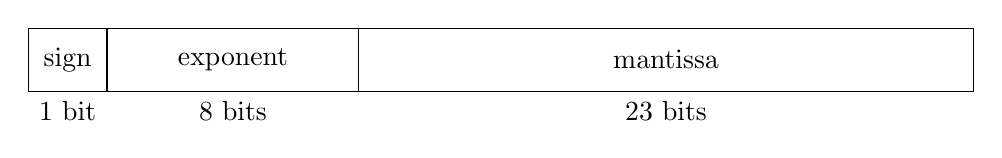
\begin{tikzpicture}
    \draw (0,0) rectangle (1,0.8);
    \draw (1,0) rectangle (4.2,0.8);
    \draw (4.2,0) rectangle (12,0.8);

    \node at (0.5,0.4) {sign};
    \node at (2.6,0.4) {exponent};
    \node at (8.1,0.4) {mantissa};

    \node[below] at (0.5,0) {1 bit};
    \node[below] at (2.6,0) {8 bits};
    \node[below] at (8.1,0) {23 bits};
\end{tikzpicture}
\end{center}

\section{The Sign Bit}

The sign bit is \texttt{0} for positive numbers and \texttt{1} for negative numbers.

\begin{lstlisting}[language=Python]
if n < 0:
    sign_bit = "1"
    n = abs(n)
else:
    sign_bit = "0"
\end{lstlisting}

\section{The Exponent Field}

Single precision stores the exponent using a bias of 127.

If the actual exponent is $E$, then the stored exponent is:

\[
E + 127
\]

For example, if $E = 7$, then:

\[
E_{\text{stored}} = 7 + 127 = 134
\]

Then 134 is converted to an 8-bit binary number.

\begin{lstlisting}[language=Python]
exp = int(exponent) + 127
exp_binary_rep = convert_integer_to_binary(exp)
\end{lstlisting}

If the exponent binary representation has fewer than 8 bits, we pad with leading zeroes:

\begin{lstlisting}[language=Python]
if len(exp_binary_rep) < 8:
    exp_binary_rep = (8 - len(exp_binary_rep)) * "0" + exp_binary_rep
\end{lstlisting}

\section{Final 32-Bit String}

Finally, the 32-bit representation is assembled as:

\[
\text{sign bit} + \text{exponent bits} + \text{mantissa bits}
\]

\begin{lstlisting}[language=Python]
float_rep = sign_bit + exp_binary_rep + mantissa
\end{lstlisting}

\section{Complete Program}

\begin{lstlisting}[language=Python]
def convert_integer_to_binary(num):
    # Convert a nonnegative integer to a binary string.

    if num == 0:
        return "0"

    result = ""

    while num > 0:
        digit = num % 2
        result = str(digit) + result
        num = num // 2

    return result


def convert_fraction_to_binary(num, places):
    # Convert a fractional number between 0 and 1 to binary.

    result = ""
    count = 0

    while num > 0 and count < places:
        comparison = 2 ** (-(count + 1))

        if num >= comparison:
            result = result + "1"
            num = num - comparison
        else:
            result = result + "0"

        count = count + 1

    while len(result) < places:
        result = result + "0"

    return result


def get_binary_rep(n, p):
    # Return binary representation of n using p fractional places.

    front = int(n)
    back = n - front

    front_bin = convert_integer_to_binary(front)
    back_bin = convert_fraction_to_binary(back, p)

    return front_bin + "." + back_bin


def normalize_binary_rep(front_bin, back_bin):
    # Return exponent and mantissa bits from binary pieces.

    if front_bin != "0":
        exponent = len(front_bin) - 1
        mantissa = front_bin[1:] + back_bin
    else:
        first_one = back_bin.find("1")

        if first_one == -1:
            exponent = 0
            mantissa = "0" * 23
        else:
            exponent = -(first_one + 1)
            mantissa = back_bin[first_one + 1:]

    if len(mantissa) < 23:
        mantissa = mantissa + (23 - len(mantissa)) * "0"

    if len(mantissa) > 23:
        mantissa = mantissa[0:23]

    return exponent, mantissa


def get_32_bit_float_rep(n, p):
    # Construct a simplified 32-bit floating point representation.

    if n < 0:
        sign_bit = "1"
        n = abs(n)
    else:
        sign_bit = "0"

    front = int(n)
    back = n - front

    front_bin = convert_integer_to_binary(front)
    back_bin = convert_fraction_to_binary(back, p)

    exponent, mantissa = normalize_binary_rep(front_bin, back_bin)

    exp = exponent + 127
    exp_binary_rep = convert_integer_to_binary(exp)

    if len(exp_binary_rep) < 8:
        exp_binary_rep = (8 - len(exp_binary_rep)) * "0" + exp_binary_rep

    if len(exp_binary_rep) > 8:
        raise ValueError("Exponent does not fit in 8 bits.")

    return sign_bit + exp_binary_rep + mantissa


n = float(input("Enter your floating point value: "))
p = int(input("Enter the number of binary places in the result: "))

binary_rep = get_binary_rep(abs(n), p)
float_rep = get_32_bit_float_rep(n, p)

print("Binary representation:", binary_rep)
print("32-bit floating point representation:", float_rep)
print("Grouped:")
print(float_rep[0], float_rep[1:9], float_rep[9:])
\end{lstlisting}

\section{Testing the Program}

For:

\[
n = 3.125
\]

we know:

\[
3.125_{10} = 11.001_2
\]

Normalized:

\[
11.001_2 = 1.1001_2 \times 2^1
\]

So:

\begin{itemize}
    \item sign bit is \texttt{0};
    \item exponent is $1$;
    \item biased exponent is $1+127 = 128$;
    \item exponent bits are \texttt{10000000};
    \item mantissa begins \texttt{1001} and is padded with zeroes.
\end{itemize}

Thus the 32-bit representation should be:

\[
0\ 10000000\ 10010000000000000000000
\]

or:

\begin{lstlisting}
01000000010010000000000000000000
\end{lstlisting}

\section{Important Caveats}

This program is educational. It deliberately avoids several complications of the full IEEE-754 standard, including:

\begin{itemize}
    \item rounding instead of truncation,
    \item subnormal numbers,
    \item signed zero,
    \item infinity,
    \item NaN,
    \item overflow and underflow handling,
    \item exact binary behavior of Python's built-in floats.
\end{itemize}

Nevertheless, it captures the central idea:

\[
\text{floating point number}
=
(-1)^s \times 1.\text{mantissa} \times 2^E
\]

\section{Key Takeaways}

\begin{itemize}
    \item A floating point number can be separated into integer and fractional parts.
    \item Integer parts can be converted to binary using repeated division by 2.
    \item Fractional parts can be converted using repeated comparison to powers of $1/2$.
    \item Binary floating point numbers are normalized into the form $1.xxxxx \times 2^E$.
    \item A 32-bit representation stores 1 sign bit, 8 exponent bits, and 23 mantissa bits.
    \item The exponent is stored with a bias of 127.
    \item Python string operations are useful for constructing binary representations manually.
\end{itemize}

\end{document}
